\documentclass[12pt]{article}

%%%%%%%%%%%%%%%%%%%%%%%%%%%%%%%%%%%%%%%%%%%%%%%%%%%%%%%%%%%%%%%%%%%%%%%%%%%%%%%%
%                           Package preset for homework
%%%%%%%%%%%%%%%%%%%%%%%%%%%%%%%%%%%%%%%%%%%%%%%%%%%%%%%%%%%%%%%%%%%%%%%%%%%%%%%%
% Miscellaneous
\usepackage[margin=1in]{geometry}
\usepackage[utf8]{inputenc}
\usepackage{indentfirst}
\usepackage{blindtext}
\usepackage{graphicx}
\usepackage{xr-hyper}
\usepackage{hyperref}
\usepackage{enumitem}
\usepackage{color}
\usepackage{float}
% Math
\usepackage{latexsym}
\usepackage{amsfonts}
\usepackage{amssymb}
\usepackage{amsmath}
\usepackage{commath}
\usepackage{amsthm}
\usepackage{bbold}
\usepackage{bm}
% Physics
\usepackage{physics}
\usepackage{siunitx}
% Code typesetting
\usepackage{listings}
% Citation
\usepackage[authoryear]{natbib}
\usepackage{appendix}
\usepackage[capitalize]{cleveref}
% Title & name
\title{Homework}
\author{Tien Vo}
\date{\today}


%%%%%%%%%%%%%%%%%%%%%%%%%%%%%%%%%%%%%%%%%%%%%%%%%%%%%%%%%%%%%%%%%%%%%%%%%%%%%%%%
%                   User-defined commands and environments
%%%%%%%%%%%%%%%%%%%%%%%%%%%%%%%%%%%%%%%%%%%%%%%%%%%%%%%%%%%%%%%%%%%%%%%%%%%%%%%%
%%% Misc
\sisetup{load-configurations=abbreviations}
\newcommand{\due}[1]{\date{Due: #1}}
\newcommand{\hint}{\textit{Hint}}
\let\oldt\t
\renewcommand{\t}[1]{\text{#1}}

%%% Bold sets & abbrv
\newcommand{\N}{\mathbb{N}}
\newcommand{\Z}{\mathbb{Z}}
\newcommand{\R}{\mathbb{R}}
\newcommand{\Q}{\mathbb{Q}}
\let\oldP\P
\renewcommand{\P}{\mathbb{P}}
\newcommand{\LL}{\mathcal{L}}
\newcommand{\FF}{\mathcal{F}}
\newcommand{\HH}{\mathcal{H}}
\newcommand{\NN}{\mathcal{N}}
\newcommand{\ZZ}{\mathcal{Z}}
\newcommand{\RN}[1]{\textup{\uppercase\expandafter{\romannumeral#1}}}
\newcommand{\ua}{\uparrow}
\newcommand{\da}{\downarrow}

%%% Unit vectors
\newcommand{\xhat}{\vb{\hat{x}}}
\newcommand{\yhat}{\vb{\hat{y}}}
\newcommand{\zhat}{\vb{\hat{z}}}
\newcommand{\nhat}{\vb{\hat{n}}}
\newcommand{\rhat}{\vb{\hat{r}}}
\newcommand{\phihat}{\bm{\hat{\phi}}}
\newcommand{\thetahat}{\bm{\hat{\theta}}}

%%% Other math stuff
\providecommand{\units}[1]{\,\ensuremath{\mathrm{#1}}\xspace}
% Set new style for problem
\newtheoremstyle{problemstyle}  % <name>
        {10pt}                   % <space above>
        {10pt}                   % <space below>
        {\normalfont}           % <body font>
        {}                      % <indent amount}
        {\bfseries\itshape}     % <theorem head font>
        {\normalfont\bfseries:} % <punctuation after theorem head>
        {.5em}                  % <space after theorem head>
        {}                      % <theorem head spec (can be left empty, 
                                % meaning `normal')>

% Set problem environment
\theoremstyle{problemstyle}
\newtheorem{problemenv}{Problem}[section]
\newenvironment{problem}[1]{%
  \renewcommand\theproblemenv{#1}%
  \problemenv
}{\endproblemenv}
% Set lemma environment
\newenvironment{lemma}[2][Lemma]{\begin{trivlist}
\item[\hskip \labelsep {\bfseries #1}\hskip \labelsep {\bfseries #2.}]}{\end{trivlist}}
% Set solution environment
\newenvironment{solution}{
    \begin{proof}[Solution]$ $\par\nobreak\ignorespaces
}{\end{proof}}
\numberwithin{equation}{problemenv}

%%% Page format
\setlength{\parindent}{0.5cm}
\setlength{\oddsidemargin}{0in}
\setlength{\textwidth}{6.5in}
\setlength{\textheight}{8.8in}
\setlength{\topmargin}{0in}
\setlength{\headheight}{18pt}

%%% Code environments
\definecolor{dkgreen}{rgb}{0,0.6,0}
\definecolor{gray}{rgb}{0.5,0.5,0.5}
\definecolor{mauve}{rgb}{0.58,0,0.82}
\lstset{frame=tb,
  language=Python,
  aboveskip=3mm,
  belowskip=3mm,
  showstringspaces=false,
  columns=flexible,
  basicstyle={\small\ttfamily},
  numbers=none,
  numberstyle=\tiny\color{gray},
  keywordstyle=\color{blue},
  commentstyle=\color{dkgreen},
  stringstyle=\color{mauve},
  breaklines=true,
  breakatwhitespace=true,
  tabsize=4
}
\lstset{
  language=Mathematica,
  numbers=left,
  numberstyle=\tiny\color{gray},
  numbersep=5pt,
  breaklines=true,
  captionpos={t},
  frame={lines},
  rulecolor=\color{black},
  framerule=0.5pt,
  columns=flexible,
  tabsize=2
}


\title{Homework 8: Phys 7310 (Fall 2021)}

\begin{document}
\maketitle
%%%%%%%%%%%%%%%%%%%%%%%%%%%%%%%%%%%%%%%%%%%%%%%%%%%%%%%%%%%%%%%%%%%%%%%%%%%%%%%%
\begin{problem}{8.1}[Magnetic field in a solenoid]

(a) A right-circular solenoid of finite length $L$ and radius $a$ has $N$ turns 
per unit length and carries a current $I$. Show that the magnetic induction on 
the cylinder axis in the limit $NL\to\infty$ is
\begin{equation}
    B_z=\frac{\mu_0NI}{2}\qty(\cos\theta_1+\cos\theta_2) 
\end{equation}
where the angles are defined in the figure.

\begin{center}
    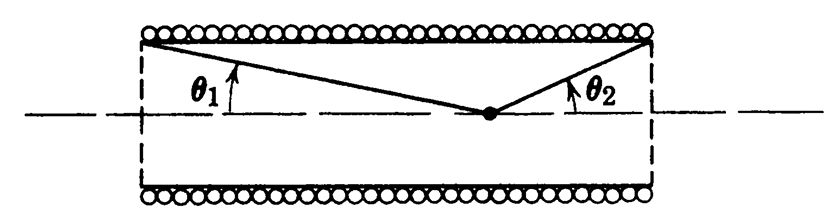
\includegraphics[width=0.7\textwidth]{hw8_p1.jpg} 
\end{center}

(b) Show that near the axis and near the (vertical) middle of the solenoid, the
magnetic field is mainly parallel to the axis, but has a small radial component,
\begin{equation}
    B_\rho\approx 24\mu_0NI\frac{a^2z\rho}{L^4} 
\end{equation}
with $L$ the length and $a$ the radius of the solenoid, and we take the vertical
center of the solenoid to be at $z=0$. You may assume the solenoid is long,
$L\gg a$. Hint: write $\cos\theta_{1,2}$ in terms of $L,a$, and $z$ and find an
expression for $B_z$ as a series. How can you relate $B_z$ to $B_\rho$?

(c) Using similar methods, again assuming a long solenoid $L\gg a$, show that at
the end of the solenoid, the magnetic field near the axis has components
\begin{equation}
    B_z\approx\frac{\mu_0NI}{2}\qquad\text{and}\qquad
    B_\rho\approx\pm\frac{\mu_0NI}{4}\frac{\rho}{a}
\end{equation}
where the two signs are for the two ends of the cylinder (you need only check
one).
\begin{solution}
(a) First we find the magnetic field due to a single loop of current $I$
with radius $a$ located at $z=z_0$. The only component is in the $\phihat$
direction. So we can write the volume current density in cylindrical 
coordinates as
\begin{equation}
    \vb{J}=I\delta(r'-a)\delta(z'-z_0)\phihat 
\end{equation}
such that the current through a small Amperian area $da'=dr'dz'$ perpendicular 
to the loop is
\begin{equation}
    \int da'J_\phi=I\int dr'dz'\delta(r'-a)\delta(z'-z_0)=I
\end{equation}

Now, from Biot-Savart law, the magnetic field due to this current on the $z$
axis is
\begin{align}
    \vb{B}_0
    &=\frac{\mu_0}{I}{4\pi}\int_0^\infty\int_0^{2\pi}\int_{-\infty}^\infty 
        r'dr'd\phi'dz'\delta(r'-a)\delta(z'-z_0)
        \phihat\times\frac{\vb{x}-\vb{x}'}{\abs{\vb{x}-\vb{x}'}^3}\notag\\
    &=\frac{\mu_0I}{4\pi}\int_0^\infty\int_0^{2\pi}\int_{-\infty}^\infty 
        r'dr'd\phi'dz'\delta(r'-a)\delta(z'-z_0)
        \frac{(z-z')\cos\phi'\xhat+(z-z')\sin\phi'\yhat+r'\zhat}
            {[r'^2+(z-z')^2]^{3/2}}\notag\\
    &=\frac{\mu_0I}{2}\int_0^\infty\int_{-\infty}^\infty
    \frac{r'^2\delta(r'-a)\delta(z'-z_0)dr'dz'}{[r'^2+(z-z')^2]^{3/2}}\zhat\notag\\
    &=\frac{\mu_0I}{2}\frac{a^2}{[a^2+(z-z_0)^2]^{3/2}}\zhat
\end{align}
where the $x$ and $y$ components have dropped out in the azimuthal integration
due to azimuthal symmetry on the $z$ axis. Now, when $NL\to\infty$, the density
of loops $n'$ is high enough that it can be written in differentials as
$dn'=Ndz'$. We can now consider the contribution due to multiple loops placed 
from $z_0=0\to L$
\begin{align}\label{p1a:B}
    \vb{B}
    &=\int d\vb{B}_0\notag\\
    &=\frac{\mu_0NI}{2}a^2\int_0^L\frac{dz_0}{[a^2+(z-z_0)^2]^{3/2}}\zhat\notag\\
    &=\frac{\mu_0NI}{2}\qty[\frac{z}{\sqrt{a^2+z^2}}+\frac{L-z}{\sqrt{a^2+(L-z)^2}}]\zhat\notag\\
    &=\frac{\mu_0NI}{2}\qty[\cos\theta_1+\cos\theta_2]\zhat
\end{align}
where $\theta_{1,2}$ are defined as drawn in the figure.

(b) By a translation $z\mapsto z+L /2$, we can rewrite \eqref{p1a:B} as
\begin{align}
    B_z
    &=\frac{\mu_0NI}{2}\qty[\frac{L-2z}{4a^2+(L-2z)^2}+\frac{L+2z}{\sqrt{4a^2+(L+2z)^2}}]\notag\\
    &=\frac{\mu_0NI}{2}\qty[\frac{1-2z/L}{\sqrt{4(a/L)^2+(1-2z/L)^2}}+\frac{1+2z/L}{\sqrt{4(a/L)^2+(1+2z/L)^2}}]
\end{align}
Using Mathematica, we can expand $B_z$ around small $z /L$ and $a /L$
\begin{equation}
    B_z\approx\mu_0NI\qty(1-2\frac{a^2}{L^2})-24\mu_0NI\frac{z^2}{L^2}\frac{a^2}{L^2} 
\end{equation}
Now, since $\div{\vb{B}}=0$, we can write the differential equation
\begin{equation}\label{p1b:diffeq}
    \frac1\rho\frac{\partial}{\partial\rho}\qty(\rho B_\rho)+\frac{\partial
    B_z}{\partial z}=0 
\end{equation}
Note that since $\partial B_z /\partial z\neq 0$, $B_\rho$ has to be non-zero.
The solution to \eqref{p1b:diffeq} is, according to Mathematica,
\begin{equation}
    B_\rho=-\frac{\rho}{2}\frac{\partial B_z}{\partial
    z}=24\mu_0NI\frac{z\rho}{L^2}\frac{a^2}{L^2} 
\end{equation}

(c) Let us now rewriting \eqref{p1a:B} again without applying any translation
\begin{align}
    B_z
    &=\frac{\mu_0NI}{2}\qty[\frac{1-z/L}{\sqrt{(a/L)^2+(1-z/L)^2}}+\frac{z/L}{\sqrt{(a/L)^2+(z/L)^2}}]
    \notag\\
    &\approx\frac{\mu_0NI}{2}\qty[1-\frac12\frac{a^2}{L^2}+\frac{z}{a}]\notag\\
    &\approx\frac{\mu_0NI}{2}
\end{align}
To find the small radial component, we have to retain the first-order term in
$z$
\begin{equation}
    B_\rho=-\frac{\rho}{2}\frac{\partial B_z}{\partial
    z}\approx-\frac{\mu_0NI}{4}\frac{\rho}{a} 
\end{equation}
\end{solution}
\end{problem}
%%%%%%%%%%%%%%%%%%%%%%%%%%%%%%%%%%%%%%%%%%%%%%%%%%%%%%%%%%%%%%%%%%%%%%%%%%%%%%%%    
%%%%%%%%%%%%%%%%%%%%%%%%%%%%%%%%%%%%%%%%%%%%%%%%%%%%%%%%%%%%%%%%%%%%%%%%%%%%%%%%
\begin{problem}{8.2}[Rotating sphere]
A sphere of radius $a$ carries a uniform surface-charge distribution $\sigma$.
The sphere is rotated about a diameter with constant angular velocity $\omega$.
Find the vector potential and magnetic-flux density both inside and outside the
sphere.
\begin{solution}
From Griffiths, we can write the volume current density from the surface current
density $\vb{K}=\sigma\vb{v}=\sigma\omega a\sin\theta\phihat$ as
\begin{equation}
    \vb{J}=\vb{K}\delta(r'-a) 
    =\sigma\omega a\sin\theta\delta(r'-a)\phihat
\end{equation}
Then the vector potential is
\begin{align}
    \vb{A}
    &=\frac{\mu_0}{4\pi}\int
    d^3x'\frac{\vb{J}(\vb{x}')}{\abs{\vb{x}-\vb{x}'}}\notag\\
    &=\mu_0\sigma\omega a\sum_{l,m}\frac1{2l+1}Y_{lm}(\Omega)\int d^3x'
    \frac{r_<^l}{r_>^{l+1}}
    \delta(r'-a)\sin\theta'(-\sin\phi'\xhat+\cos\phi'\yhat)
    Y_{lm}^\ast(\Omega')\notag\\
    &=\mu_0\sigma\omega
    a\sum_{l,m}\sqrt{\frac{1}{4\pi(2l+1)}\frac{(l-m)!}{(l+m)!}}Y_{lm}(\Omega)
    \int_0^\infty \frac{r'^2r_<^l}{r_>^{l+1}}\delta(r'-a)dr'\notag\\
    &\qquad\times\int_0^\pi\sin^2\theta'P_l^m(\cos\theta')d\theta'
        \int_0^{2\pi}e^{-im\phi'}(-\sin\phi'\xhat+\cos\phi'\yhat)d\phi'
\end{align}
The azimuthal integration vanishes for $m^2\neq 1$. Thus, the vector potential
now becomes
\begin{align}
    \vb{A}
    &=\mu_0\sigma\omega a\sum_{l=1}^\infty
    \frac{1}{\sqrt{4\pi(2l+1)}}R_l\pi\sqrt{\frac{(l-1)!}{(l+1)!}}
    \int_0^\pi\sin^2\theta'P_l^1(\cos\theta')d\theta'
\qty[Y_{l,1}(i\xhat+\yhat)+Y_{l,1}^\ast(-i\xhat+\yhat)]
\end{align}
where $R_l$ is the radial integration. Note also that
\begin{align}
    \int_0^\pi\sin^2\theta'P_l^1(\cos\theta')d\theta'
    =\int_{-1}^1\sqrt{1-x^2}P_l^1(x)dx
    =-\int_{-1}^1(1-x^2)P_l'(x)dx
    =-\frac43
\end{align}
only for $l=1$. Then the vector potential simplifies to
\begin{align}
    \vb{A}
    &=-\frac43\sqrt{\frac{\pi}{24}}\mu_0\sigma\omega
    aR_1\qty[i(Y_{1,1}-Y_{1,1}^\ast)\xhat+(Y_{1,1}+Y_{1,1}^\ast)\yhat]\notag\\
    &=\frac13\mu_0\sigma\omega a\sin\theta
    R_1(-\sin\phi\xhat+\cos\phi\yhat)\notag\\
    &=\frac13\mu_0\sigma\omega a\sin\theta R_1\phihat
\end{align}
The radial integral evaluates to
\begin{subequations}
    \begin{align}
        R_1(r'>r)&=r\int_0^\infty\delta(r'-a)dr'=r\\
        R_1(r'<r)&=\int_0^\infty\frac{r'^3}{r^2}\delta(r'-a)dr'
        =\frac{a^3}{r^2}
    \end{align} 
\end{subequations}
Then we can write the final solution as
\begin{subequations}
    \begin{align}
        \vb{A}_{r'<r}&=\frac{\mu_0\sigma\omega}{3} ar\sin\theta\phihat\\
        \vb{A}_{r'>r}&=\frac{\mu_0\sigma\omega}{3}\frac{a^4}{r^2}\sin\theta\phihat
    \end{align} 
\end{subequations}
Then since $\vb{B}=\curl{\vb{A}}$, it follows that
\begin{subequations}
    \begin{align}
        \vb{B}_{r'<r}&=\frac23\mu_0\sigma\omega
        a\qty(\cos\theta\rhat-\sin\theta\thetahat)\\
        \vb{B}_{r'>r}&=\frac13\mu_0\sigma\omega\frac{a^4}{r^3}\qty(2\cos\theta\rhat+\sin\theta\thetahat)
    \end{align} 
\end{subequations}
\end{solution}
\end{problem}
%%%%%%%%%%%%%%%%%%%%%%%%%%%%%%%%%%%%%%%%%%%%%%%%%%%%%%%%%%%%%%%%%%%%%%%%%%%%%%%%
%%%%%%%%%%%%%%%%%%%%%%%%%%%%%%%%%%%%%%%%%%%%%%%%%%%%%%%%%%%%%%%%%%%%%%%%%%%%%%%%
\begin{problem}{8.3}[Image current]
A current distribution $\vb{J}(\vb{r})$ exists in a medium of unit relative
permeability adjacent to a semi-infinite slab of material having relative
permeability $\mu_r$ and filling the half-space, $z<0$.

(a) Show that for $z>0$ the magnetic induction can be calculated by replacing
the medium of permeability $\mu_r$ by an image current distribution,
$\vb{J}^\ast$, with components
\begin{equation}
    \qty(\frac{\mu_r-1}{\mu_r+1})J_x(x,y,-z),
    \qquad
    \qty(\frac{\mu_r-1}{\mu_r+1})J_y(x,y,-z),
    \qquad
    -\qty(\frac{\mu_r-1}{\mu_r+1})J_z(x,y,-z)
\end{equation}

(b) Show that for $z<0$ the magnetic induction appears to be due to a current
distribution $[2\mu_r /(\mu_r+1)]\vb{J}$ in a medium of unit relative
permeability.
\begin{solution}
(a,b) Suppose that the magnetic field in both half-infinite regions is given by
the indicated currents. Then we can write
\begin{subequations}\label{p3:B}
    \begin{align}
        \vb{B}_{z\geq0}
        &=\frac{\mu_0}{4\pi}\int
        d^3x'\qty[\vb{J}(\vb{x}')+\vb{J}^\ast(\vb{x}')]\times\frac{\vb{x}-\vb{x}'}{\abs{\vb{x}-\vb{x}'}^3}\\
        \vb{B}_{z<0}
        &=\frac{\mu_0}{4\pi}\frac{2\mu_r}{\mu_r+1}
        \int d^3x'\vb{J}(\vb{x}')\times\frac{\vb{x}-\vb{x}'}{\abs{\vb{x}-\vb{x}'}^3}
    \end{align} 
\end{subequations}
where the position vector can be splitted into two terms
$\vb{x}=\vb{x}_\bot+z\zhat$ where $\vb{x}_\bot=x\xhat+y\yhat$ and
\begin{equation}
    \vb{J}^\ast(\vb{x}_\perp,z) 
    =\frac{\mu_r-1}{\mu_r+1}\qty[\vb{J}_\bot(\vb{x}_\bot,-z)-J_z(\vb{x}_\bot,-z)\zhat]
\end{equation}
Now, we need only show that the magnetic field \eqref{p3:B} follows  
$\div{\vb{B}}=0$ and Ampere's Law, or
\begin{equation}
    \lim_{z\to0^-}\vb{B}\vdot\zhat=\lim_{z\to0^+}\vb{B}\vdot\zhat 
    \qquad\text{and}\qquad
    \lim_{z\to0^-}\vb{B}\times\zhat=\mu_r\lim_{z\to0^+}\vb{B}\times\zhat
\end{equation}
because we let the normal vector to the boundary between the two material be in 
the $\zhat$ direction.

First, let us consider the former condition
\begin{align}
    \lim_{z\to0^+}\vb{B}\vdot\zhat
    &=\frac{\mu_0}{4\pi}\Bigg\{\int\frac{d^3x'}{\abs{\vb{x}_\bot-\vb{x}'}^3}
        \qty[(y-y')J_x(\vb{x}_\bot',z')-(x-x')J_y(\vb{x}_\bot',z')]\notag\\
    &\qquad+\int\frac{d^3x'}{\abs{\vb{x}_\bot-\vb{x}'}^3}
        \qty[(y-y')J_x^\ast(\vb{x}_\bot',z')-(x-x')J_y^\ast(\vb{x}_\bot',z')]
\Bigg\}\notag\\
    &=\frac{\mu_0}{4\pi}\Bigg\{\int\frac{d^3x'}{\abs{\vb{x}_\bot-\vb{x}'}^3}
        \qty[(y-y')J_x(\vb{x}_\bot',z')-(x-x')J_y(\vb{x}_\bot',z')]\notag\\
    &\qquad+\frac{\mu_r-1}{\mu_r+1}\int\frac{d^3x'}{\abs{\vb{x}_\bot-\vb{x}'}^3}
        \qty[(y-y')J_x(\vb{x}_\bot',-z')-(x-x')J_y(\vb{x}_\bot',-z')]
\Bigg\}
\end{align}

Let $\overline{z}'=-z'$ in the second integration. Then $\int_{-\infty}^\infty
dz'=-\int_{\infty}^{-\infty}d\overline{z}'=\int_{-\infty}^\infty
d\overline{z}'$. Also,
$\abs{\vb{x}_\bot-\vb{x}'}=\sqrt{(x-x')^2+(y-y')^2+\overline{z}'^2}$. So the
first terms in the integral are not affected and we can write
\begin{align}
    \lim_{z\to0^+}\vb{B}\vdot\zhat
    &=\frac{\mu_0}{4\pi}\Bigg\{
        \int\frac{d^3x'}{\abs{\vb{x}_\bot-\vb{x}'}^3}
        \qty[(y-y')J_x(\vb{x}_\bot',z')-(x-x')J_y(\vb{x}_\bot',z')]\notag\\
    &\qquad+\frac{\mu_r-1}{\mu_r+1}
    \int\frac{d^3x'}{\abs{\vb{x}_\bot-\vb{x}'}^3}\qty[
        (y-y')J_x(\vb{x}_\bot',z')-(x-x')J_y(\vb{x}_\bot',z') 
    ]\Bigg\}\notag\\
    &=\frac{\mu_0}{4\pi}\frac{2\mu_r}{\mu_r+1}
    \int\frac{d^3x'}{\abs{\vb{x}_\bot-\vb{x}'}^3}\qty[(y-y')J_x(\vb{x}_\bot',z')-(x-x')J_y(\vb{x}_\bot',z')]\notag\\
    &=\frac{\mu_0}{4\pi}\frac{2\mu_r}{\mu_r+1}
    \int\frac{d^3x'}{\abs{\vb{x}_\bot-\vb{x}'}^3}\qty[\vb{J}(\vb{x}')\times(\vb{x}_\bot-\vb{x}')]\vdot\zhat\notag\\
    &=\lim_{z\to0^-}\vb{B}\vdot\zhat
\end{align}
So the first condition is satisfied. Now, consider the second one
\begin{align}
    \mu_r\lim_{z\to0^+}\vb{B}\times\zhat 
    &=\frac{\mu_0\mu_r}{4\pi}\int\frac{d^3x'}{\abs{\vb{x}_\bot-\vb{x}'}^3}
    \qty[\qty(\vb{J}+\vb{J}^\ast)\times(\vb{x}_\bot-\vb{x}')]\times\zhat\notag\\
    &=\frac{\mu_0\mu_r}{4\pi}\Bigg\{
        \int\frac{d^3x'}{\abs{\vb{x}_\bot-\vb{x}'}^3}
        \Bigg[[(x-x')J_z+z'J_x]\xhat+[(y-y')J_z+z'J_y]\yhat\Bigg]\notag\\
    &\qquad+\frac{\mu_r-1}{\mu_r+1}
        \int\frac{d^3x'}{\abs{\vb{x}_\bot-\vb{x}'}^3}
        \Bigg[[-(x-x')J_z+z'J_x]\xhat+[-(y-y')J_z+z'J_y]\yhat\Bigg]
    \Bigg\}
\end{align}
By letting $z'\to-z'$ in the second integral, we get
\begin{align}
    \mu_r\lim_{z\to0^+}\vb{B}\times\zhat
    &=\frac{\mu_0}{4\pi}\frac{2\mu_r}{\mu_r+1}
        \int\frac{d^3x'}{\abs{\vb{x}_\bot-\vb{x}'}^3}
        \Bigg[[(x-x')J_z+z'J_x]\xhat+[(y-y')J_z+z'J_y]\yhat\Bigg]\notag\\
    &=\frac{\mu_0}{4\pi}\frac{2\mu_r}{\mu_r+1}
        \int\frac{d^3x'}{\abs{\vb{x}_\bot-\vb{x}'}^3}
        \qty[\vb{J}\times(\vb{x}_\bot-\vb{x}')]\times\zhat\notag\\
    &=\lim_{z\to0^-}\vb{B}\times\zhat
\end{align}
Thus, \eqref{p3:B} follows all boundary conditions.
\end{solution}
\end{problem}
%%%%%%%%%%%%%%%%%%%%%%%%%%%%%%%%%%%%%%%%%%%%%%%%%%%%%%%%%%%%%%%%%%%%%%%%%%%%%%%%
\end{document}
